% UGEN — conference manuscript.
% Self-contained: compiles with a standard TeX install (tested with tectonic), using only
% widely available packages. To submit to a specific venue, replace the preamble block
% marked "CONFERENCE STYLE" with that venue's class/style, e.g.:
%     \documentclass{article}\usepackage[final]{neurips_2024}
%     \documentclass{article}\usepackage{iclr2025_conference,times}
% and delete the geometry/font lines below. Body, tables, figure, and bibliography are
% venue-agnostic.

% ===================== CONFERENCE STYLE (swap for venue class) =====================
\documentclass[10pt]{article}
\usepackage[letterpaper,margin=1in]{geometry}
\usepackage{times}
% ==================================================================================

\usepackage[utf8]{inputenc}
\usepackage[T1]{fontenc}
\usepackage{amsmath,amssymb}
\usepackage{booktabs}
\usepackage{graphicx}
\usepackage{caption}
\usepackage[hidelinks]{hyperref}
\usepackage{xcolor}
\usepackage[round]{natbib}
\usepackage{microtype}

\title{\bfseries Consistency Is the Only Signal That Transfers:\\
A Preregistered Three-Lineage Map of Cheap Uncertainty Signals\\
in Small Instruct Models}
\author{Anonymous submission}
\date{}

\begin{document}
\maketitle

\begin{abstract}
Practitioners routinely estimate whether a language model's answer is correct from cheap,
inference-time signals: verbalized confidence, token log-probabilities, token-level entropy,
or agreement across resampled generations. We preregistered five predictions about what these
signals measure and tested them on a frozen protocol---13 standard benchmarks across five
domains, ${\sim}200$ items each, identical prompts, one shared extraction module---in three
independent 3--4B instruct lineages (Qwen2.5-3B, Llama-3.2-3B, Gemma-3-4B). Most predictions
failed, and the failures organize into a sharper map. (1) $K$-sample answer consistency
($K{=}5$) discriminates correctness at AUROC $.740/.746/.756$ across the three lineages---the
only signal whose performance transfers. (2) Every token-level signal is lineage-specific:
mean log-probability ranges from mildly useful ($.61$) to below chance ($.39$); token entropy
from $.61$ to chance. (3) Verbalized confidence has three phenotypes---collapsed
(${\sim}96\%$ ``100'', robust to four elicitation wordings including an inverted scale),
graded-informative ($.615$), and compressed-high ($.605$). (4) An information decomposition
explains the structure: $I(\text{consistency};\text{correctness}\mid\text{entropy})$ exceeds
its shuffled-control floor in $12/12$ model$\times$domain cells, while
$I(\text{entropy};\text{correctness}\mid\text{consistency})$ does so in only $2/12$---
uncertainty information lives in the distribution over \emph{outcomes}, not over \emph{tokens};
the two entropies are nearly uncorrelated ($\rho = -.05$ to $.31$). (5) Mechanistically,
consistency behaves like a measure of generation-basin depth: single-path agreement is more
reliable than divergent-path agreement ($.87$--$.88$ vs $.70$--$.78$), and its failure mode is
a distinct population of convergent misconceptions (6--10\% of items, precision ceiling
${\approx}.85$--$.88$ at full agreement) concentrated on plausibility-shaped benchmarks.
\end{abstract}

\section{Introduction}
When a deployed language model answers a question, the deployer's first practical question is:
\emph{should I trust this one?} Full solutions---training probes, ensembles of models,
retrieval verification---are often unavailable at inference time. What remain are cheap signals
computable from the model's own generation: ask the model how confident it is; read the
log-probability or entropy of the tokens it produced; or sample $K$ additional generations and
count agreement.

These signals are used interchangeably as ``model uncertainty,'' and the literature evaluates
them mostly one model family at a time. Whether a signal validated on one lineage means the
same thing on another is rarely tested, and the question of what each signal \emph{measures}---
as opposed to how well it scores on one benchmark---is usually left implicit.

We approached this as a measurement problem with a preregistered design. Before data collection
we froze: five falsifiable predictions (P1--P5) inherited from a pilot study on a custom
benchmark; a 13-benchmark, five-domain evaluation suite with per-item frozen prompts; a single
measurement protocol (greedy chain-of-thought pass, $K{=}5$ resampling at temperature $0.7$,
one fixed confidence elicitation); exclusion rules (accuracy outside $[.10,.90]$; extraction
failure ${>}10\%$ per cell); and the statistical machinery (bootstrap CIs on everything,
permutation tests with Holm correction for the primary family, shuffled-control floors under
every plug-in information estimate). We then ran the frozen protocol on three independent model
lineages at matched scale.

\paragraph{Contributions.}
\begin{enumerate}\itemsep2pt
\item A preregistered, QC-disciplined map of four cheap uncertainty-signal families $\times$ 13
benchmarks $\times$ 3 model lineages (7{,}620 measured items), with all raw rows, code, and
generated tables released.
\item The finding that \textbf{only behavioral consistency transfers across lineages}
(AUROC $.74$--$.76$ in all three), while token-level signals vary from useful to
anti-predictive and verbalized confidence splits into three lineage phenotypes---one of which
(total collapse) we show is robust to four elicitation wordings.
\item An information-theoretic decomposition establishing that consistency contains
correctness information that token entropy does not ($12/12$ cells), while the converse fails
($10/12$)---i.e., ``uncertainty'' factorizes into an outcome-level quantity that tracks
correctness and a token-level quantity that mostly does not.
\item A mechanistic characterization: consistency reads the depth of the generation basin
(single-path agreement $>$ divergent-path agreement), and its residual errors are convergent
misconceptions---a structured, benchmark-localized population, not noise.
\end{enumerate}

\section{Related work}
\paragraph{Verbalized confidence.} Language models can be prompted to state confidence in words
or numbers \citep{lin2022teaching,kadavath2022know,tian2023calibration}. Findings there are
dominated by larger models; our results show that at 3--4B the very \emph{existence} of a graded
verbal signal is lineage-dependent.

\paragraph{Self-consistency and resampling.} \citet{wang2023selfconsistency} introduced majority
voting over sampled chains to improve accuracy; subsequent work uses agreement as a confidence
proxy. We measure what that proxy contains, relative to and conditional on other signals.

\paragraph{Semantic entropy and generation-level uncertainty.} \citet{kuhn2023semantic} and
\citet{farquhar2024semantic} argue for uncertainty measured over meanings rather than tokens.
Our answer-distribution/token-distribution dissociation ($\rho$ down to $-.05$; AUROC $.70$ vs
$.49$ in the same model) is a within-protocol, cross-lineage confirmation of that program's
central premise, obtained with exact-match answer equivalence rather than entailment clustering.

\paragraph{Calibration of neural networks.} \citet{guo2017calibration} established the modern
calibration toolkit (ECE, temperature scaling); we report quantile-binned ECE/Brier alongside
discrimination and keep the two questions separate.

\paragraph{Benchmarks.} MMLU \citep{hendrycks2021mmlu}, MMLU-Pro \citep{wang2024mmlupro},
TruthfulQA \citep{lin2022truthfulqa}, GSM8K \citep{cobbe2021gsm8k}, SVAMP
\citep{patel2021svamp}, MultiArith \citep{roy2015arithmetic}, CommonsenseQA
\citep{talmor2019commonsenseqa}, ARC-Challenge \citep{clark2018arc}, StrategyQA
\citep{geva2021strategyqa}, BIG-Bench Hard \citep{suzgun2022bbh}, MuSR
\citep{sprague2024musr}, HumanEval \citep{chen2021evaluating}, MBPP \citep{austin2021program}.

\paragraph{Information decomposition.} Conditional mutual information and the Williams--Beer
partial information decomposition \citep{williams2010pid} provide the machinery for the
unique-information claims; we guard the plug-in estimators with shuffled-control floors
throughout.

\section{Methods}
\paragraph{Models.} Qwen2.5-3B-Instruct, Llama-3.2-3B-Instruct, Gemma-3-4B-IT---three
independent pretraining/post-training lineages at matched scale, run fp16 on T4 GPUs with each
model's own chat template and no system prompt (byte-identical user prompts).%
\footnote{Camera-ready should cite the three model technical reports; omitted here pending
per-venue citation preferences.}

\paragraph{Benchmarks and domains.} 13 benchmarks spanning knowledge (MMLU, MMLU-Pro,
TruthfulQA), arithmetic (GSM8K, SVAMP, MultiArith), commonsense (CommonsenseQA, ARC-Challenge,
StrategyQA), reasoning (BBH 6-task subset, MuSR), and coding (HumanEval, MBPP). $n{=}200$ per
benchmark (or full split if smaller; 2{,}540 items/model), sampled once with seed 0 and frozen
to versioned JSONL with a manifest before any model ran.

\paragraph{Protocol (frozen).} Per item: (1) greedy CoT pass (512 new tokens max) with
token-level statistics---mean log-probability and mean entropy over the full chain and over the
answer span, top-1/top-2 margin, top-5 mass; (2) $K{=}5$ sampled passes ($T{=}0.7$, top-$p$
$0.9$) $\rightarrow$ consistency $=$ modal-answer fraction (code: output-agreement on
prompt-visible examples) and the answer-distribution entropy; (3) a fixed follow-up turn
eliciting confidence 0--100. One shared extraction/grading module across models (multiple-choice
letter, numeric, yes/no, executed code); unparseable answers are graded wrong and
\emph{flagged}, never dropped silently.

\paragraph{Preregistered predictions.} P1: verbal confidence discriminates on knowledge but not
arithmetic ($\Delta$AUROC $\ge .15$). P2: consistency's discrimination transfers across domains
better than confidence's. P3: full-chain log-probability is weak on arithmetic (fluency, not
correctness). P4: consistency and answer-entropy are the same signal ($\rho > .95$ everywhere;
falsified by any benchmark $< .9$). P5: a zero-cost input feature rivals internal signals where
difficulty is input-legible, and no input feature approaches confidence on knowledge.

\paragraph{QC and statistics.} Saturated cells (accuracy outside $[.10,.90]$) and cells with
${>}10\%$ extraction failure are excluded from primary contrasts; both exclusions have
flagged-included sensitivity variants. 95\% percentile bootstrap CIs on every statistic;
permutation tests (Holm-corrected within the primary family) for domain contrasts; every
MI/CMI/PID estimate is reported against the same estimator run on label-preserving shuffled
signals. Wording sensitivity of the confidence elicitation was probed post hoc under
preregistration cover (three alternative phrasings, M1, MMLU+GSM8K, $n{=}100$): probability
framing, frequency framing, and an inverted scale.

\paragraph{Independent audit.} Every headline and secondary number below was recomputed by a
second implementation sharing no code with the analysis pipeline (data integrity via SHA256,
the signal map, P4, the information asymmetry, phenotypes, QC rates, and mechanism), reading
only the frozen rows. All reproduce; details in the supplement.

\section{Results}

\subsection{The signal map}
Table~\ref{tab:signalmap} gives mean AUROC over unsaturated, extraction-clean cells.
Consistency is the best signal in essentially every benchmark$\times$model cell and its level
is lineage-stable. Token-level signals are not: Gemma's mean log-probability is anti-predictive
(below chance) on clean cells---fluent chains negatively associated with correctness---making
Gemma the only lineage where preregistered P3 was supported (arithmetic
$\text{logprob}_{\text{full}} = .297$). Verbal confidence spans three phenotypes: Qwen answers
``100'' on $95.6\%$ of items (mean confidence $.992$ when correct, $.954$ when wrong); Llama
produces a graded distribution (modal 80) at $.615$; Gemma a compressed-high distribution
($67\%$ at ``95'') at $.605$.

\begin{table}[t]
\centering
\caption{Mean AUROC (correct vs.\ incorrect) over unsaturated, extraction-clean cells.
Consistency is lineage-stable and best everywhere; token-level signals vary across lineages,
and Gemma's mean log-probability is below chance.}
\label{tab:signalmap}
\begin{tabular}{lccc}
\toprule
signal & Qwen2.5-3B & Llama-3.2-3B & Gemma-3-4B \\
\midrule
consistency ($K{=}5$)   & \textbf{.740} & \textbf{.746} & \textbf{.756} \\
verbal confidence       & .519 & .615 & .605 \\
token entropy           & .610 & .614 & .544 \\
mean log-probability    & .606 & .606 & \textbf{.391} \\
\bottomrule
\end{tabular}
\end{table}

\subsection{Preregistered verdicts}
Under strict QC, P1 is falsified in Llama ($\Delta$AUROC $= -.083$, 95\% CI $[-.152, -.019]$---
\emph{sign-reversed}: arithmetic confidence discriminates better than knowledge) and Gemma
($-.124$, $[-.192,-.052]$), and not evaluable in Qwen (the arithmetic pool empties after
exclusions; the labelled sensitivity variant gives $+.008$ $[-.040, +.040]$, falsified). P2 is
supported in Qwen and Llama, falsified in Gemma. P4 is falsified in all three lineages
(min $\rho = .001 / .009 / {-.197}$ against a predicted $> .95$). P5's preregistered falsifiers
fire in all three (Table~\ref{tab:verdicts}).

\begin{table}[t]
\centering
\caption{Preregistered predictions across the three lineages. No prediction survives in all
three; P4 fails identically in all three, and its failure mode is the central finding.}
\label{tab:verdicts}
\small
\begin{tabular}{lp{3.4cm}p{3.4cm}p{3.4cm}}
\toprule
 & Qwen2.5-3B & Llama-3.2-3B & Gemma-3-4B \\
\midrule
P1 domain gap ($\ge .15$) & inconclusive (QC); sens.\ falsified $\Delta{=}{+}.008$ & \textbf{falsified} $\Delta{=}{-}.083$ (sign-reversed) & \textbf{falsified} $\Delta{=}{-}.124$ \\
P2 consistency transfers & supported (sens.) & supported & falsified \\
P3 full-chain logprob weak on arith. & falsified ($.725$) & falsified ($.800$) & \textbf{supported} ($.297$) \\
P4 consistency $\approx$ ans.-entropy & falsified ($\rho_{\min}{\approx}.001$) & falsified ($.009$) & falsified ($-.197$) \\
P5 free-feature gate & falsified & falsified & falsified \\
\bottomrule
\end{tabular}
\end{table}

\subsection{Elicitation robustness: the collapse is the model, not the prompt}
All four wordings on Qwen produce $\ge 94\%$ modal replies with chance-level discrimination
(AUROC $.47$--$.57$, every CI spanning $.5$; parse rate $100\%$). The decisive cell is the
inverted scale: asked how likely its answer is \emph{wrong}, the model answers ``0'' ($94\%$)---
it flips the number with the semantics. The collapse is semantically coherent, genuinely held
total certainty, not number-anchoring or elicitation noncompliance.

\subsection{Information structure: outcome uncertainty, not token uncertainty}
Per model$\times$domain (never pooled), with $C=$ consistency, $E=$ answer-span token entropy,
$Y=$ correctness:
\begin{itemize}\itemsep1pt
\item $I(C;Y\mid E)$ exceeds its shuffled-control floor in $\mathbf{12/12}$ cells
($.009$--$.125$ nats, typically 10--30$\times$ floor).
\item $I(E;Y\mid C)$ does so in $\mathbf{2/12}$ cells, both marginal ($\le .02$ nats).
\item $\rho(C,E)$ ranges $-.20$ to $+.27$ across cells.
\end{itemize}
The asymmetry---consistency subsumes entropy's correctness information but not conversely---
replicates in all three lineages (Fig.~\ref{fig:entropy}). A direct comparison of the two
``entropies'' sharpens it: the entropy of the $K$-sample \emph{answer distribution} discriminates
at $.695$--$.731$ in all three models, while \emph{token-level} entropy ranges $.494$--$.706$,
and the two are nearly uncorrelated ($\rho = -.05 / .24 / .31$; Fig.~\ref{fig:entropy}A,C).
Conditioning on the best zero-cost input feature removes consistency's information in only
$2/15$ cells, both in the reasoning domain. An independent re-implementation with a
multi-permutation bias floor reproduces the asymmetry ($10/12$ vs $0/12$); the two cells where
consistency's margin does not clear the stricter floor are both the reasoning domain---the
weakest-signal domain. The direction $C \gg E$ is estimator-robust; the exact ``$12/12$''
should be read as ``in every domain except the weakest.''

\begin{figure}[t]
\centering
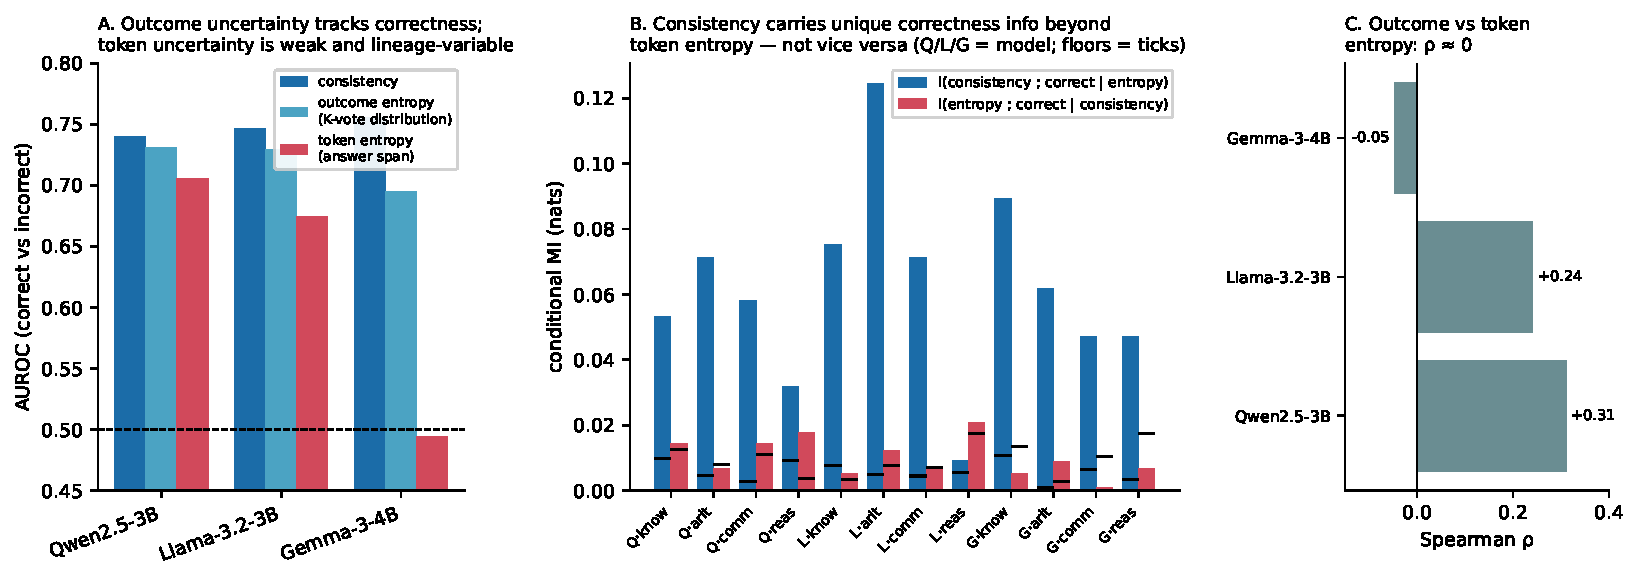
\includegraphics[width=\textwidth]{figures/entropy_vs_consistency_main.pdf}
\caption{\textbf{Entropy is not one quantity.}
(A) Consistency and the $K$-vote \emph{outcome}-entropy track correctness ($.70$--$.76$);
answer-span \emph{token}-entropy is weaker and lineage-variable (Gemma below chance).
(B) $I(C;Y\mid E)$ (blue) vs $I(E;Y\mid C)$ (red) per model$\times$domain, with
shuffled-control floors as black ticks: consistency carries unique correctness information
beyond token entropy---not vice versa.
(C) Spearman $\rho$ between outcome- and token-entropy is ${\approx}0$.}
\label{fig:entropy}
\end{figure}

\subsection{Mechanism: basin depth and convergent misconceptions}
$P(\text{correct})$ is a staircase in consistency ($C \le .4$: $.28$--$.43$; mid: $.41$--$.52$;
$C \ge .8$: $.78$--$.82$) and is flat in entropy within each band. Among high-consistency items,
agreement reached along essentially a single reasoning path is more reliable than agreement
reached along divergent paths---$.87$--$.88$ vs $.70$--$.78$ correct, in all three models. The
residual failure mode is a distinct population: wrong-but-fully-consistent items are $6.3$--
$10.4\%$ of all items (precision at $C{=}1$: $.84$--$.88$), are $91$--$97\%$ extraction-clean,
sit on prompts $1.5$--$1.9\times$ longer than average, and concentrate in TruthfulQA, MuSR,
StrategyQA, and CommonsenseQA---benchmarks shaped around plausible misconceptions. Consistency
correlates only weakly with generation length ($\rho = -.22$ to $-.34$) and prompt size
(${\approx}-.1$): it is not a repackaged difficulty feature.

\subsection{Quality control}
Cells exceeding the preregistered $10\%$ extraction-failure threshold (all excluded from primary
contrasts, all with sensitivity variants): Qwen---BBH $13.1\%$, GSM8K $12.5\%$, MMLU-Pro
$46.5\%$; Llama---MMLU-Pro $32.0\%$, MBPP $68.5\%$; Gemma---MMLU-Pro $53.0\%$, MuSR $13.1\%$,
StrategyQA $14.5\%$. Diagnosis (no parser bugs found): truncation at the frozen 512-token budget
and answer-format drift in which the preregistered fallback still recovered a graded answer.

\section{Discussion}
\paragraph{One signal, three lineages.} Of the four cheap signal families, only the $K$-sample
vote means the same thing across model families. Token-level statistics---the cheapest and
most-used proxies---change sign across lineages. A token-level uncertainty threshold tuned on
one family and shipped on another is an uncalibrated instrument; in the Gemma case it would be
systematically wrong.

\paragraph{Why P4 failed.} ``Entropy'' conflated two quantities. Uncertainty over \emph{which
tokens to emit next} is dominated by lineage-specific surface variance (phrasing, formatting,
chain length); uncertainty over \emph{which answer the process lands on when perturbed} is the
correctness-relevant part---and only resampling reads it. This is a within-protocol, exact-match
analogue of the semantic-uncertainty argument, demonstrated as a double dissociation inside a
single model (Gemma: answer-distribution entropy $.695$, token entropy $.494$, $\rho = -.05$).

\paragraph{What consistency measures.} The path-divergence result argues that consistency is a
probe of \emph{basin depth}: when the model knows, temperature perturbation barely moves the
trajectory. That framing predicts the observed failure mode---deep basins encode shared
misconceptions as readily as knowledge, so the residual errors of a consistency-gated system are
convergent misconceptions on plausibility-shaped inputs. It also explains why divergent paths
converging on one answer are \emph{weaker} evidence than a single stable path, inverting the
ensemble intuition that independent agreement is stronger.

\paragraph{Verbal confidence.} At this scale, whether graded verbal uncertainty exists at all is
a training-lineage property (three phenotypes under one protocol), and where it is absent it is
absent robustly (four wordings, semantics demonstrably understood). Claims of the form ``LLMs
can/cannot verbalize uncertainty'' need a lineage qualifier.

\paragraph{Practical guidance for 3--4B deployments.} Spend the $K$-sample budget; gate on
agreement; expect ${\approx}.85$ precision at full agreement; and treat the remaining errors as
misconception-shaped, not noise. Token statistics should be used only with per-lineage
validation, and verbal confidence only after checking the lineage produces one.

\section{Limitations}
Three lineages at 3--4.3B; findings may not extend to frontier scale. Single seed so far (the
preregistered seed run is built but unexecuted; all claims carry that caveat). The frozen
512-token budget truncates verbose models on long-form benchmarks---flagged, excluded from
primary contrasts, and diagnosed. $K{=}5$ is small; consistency at $.74$--$.76$ is likely a
floor. Exact-match/execution grading is conservative. MI/CMI/PID are plug-in estimates guarded
by shuffled controls, not debiased estimators. GPQA was inaccessible (gated). Contamination of
older benchmarks is plausible; we measure uncertainty--correctness relationships, not capability.

\section{Reproducibility}
Everything derives from: frozen benchmark JSONLs with manifest; a frozen measurement protocol,
audited by a smoke test per model before any full run; raw rows committed per session with an
append-only kernel audit trail; a SHA256-manifested master dataset; analyses that read only
frozen rows and emit every table/figure cited here; a timestamped deviations log; and an
independent second-implementation audit of every reported number. The preregistration predates
all data.

\bibliographystyle{plainnat}
\bibliography{references}

\end{document}
